%!TEX root = ../../report.tex
\section{Mapping with Location noise}

\subsection{Monte Carlo localization}

AMCL

Scan map with location noise and AMCL
Considerations on noise. What types of noise are present. Estimation of the noise. Comparison between estimation and actual error (of bags) 
Non-ideal Inverse Sensor Model
From hector

\subsection{Monte Carlo Integration Inverse Sensor Model}

\cite{monteCarloIntegration}

Cone Sensor Model
Based on sonar model. Used to incorporate pose noise. 
Simulation of Mapping with Location Noise
Comparison
Efficiency - Computational price
Map Score (obstacle centered and whole map, adjusted for number of cells)
\begin{figure}
	\centering
	\includegraphics[width=0.7\linewidth]{figures/static_mapping/particle_sensor}
	\caption{Example map with few scans from the five highest weighted particles.}
	\label{fig:particle_sensor}
\end{figure}

\begin{figure}
	\centering
	\begin{subfigure}[b]{0.45\textwidth}
		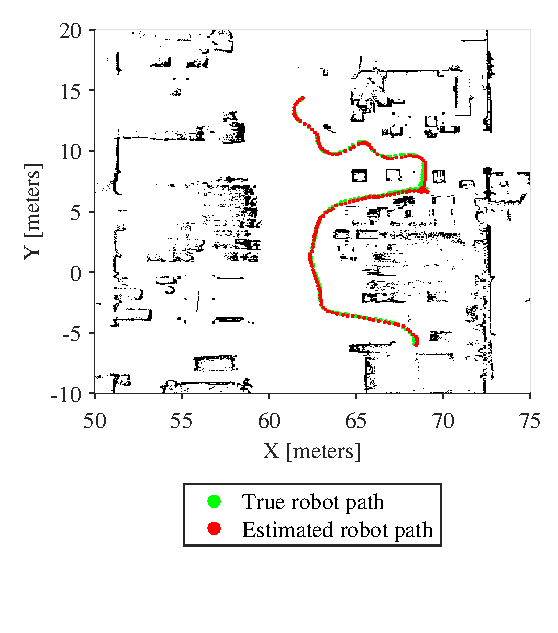
\includegraphics[width=\textwidth]{figures/static_mapping/map_with_poses}
		\caption{World represenation}
		\label{fig:simulated_robot_estimate_total}
	\end{subfigure}
	~ %add desired spacing between images, e. g. ~, \quad, \qquad, \hfill etc. 
	%(or a blank line to force the subfigure onto a new line)
	\begin{subfigure}[b]{0.45\textwidth}
		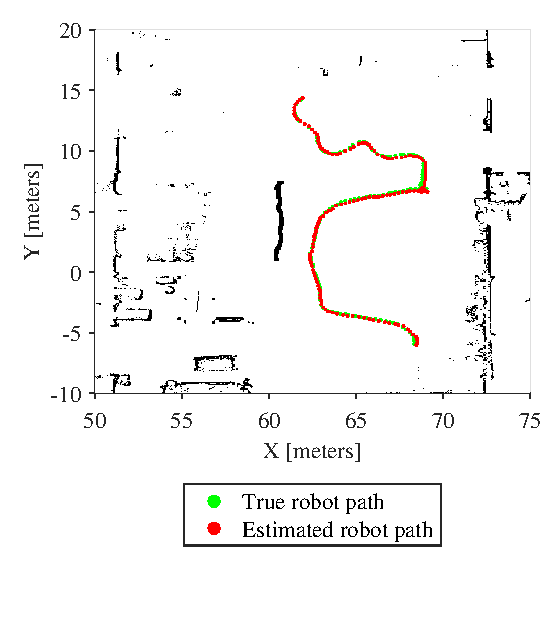
\includegraphics[width=\textwidth]{figures/static_mapping/amcl_map_with_poses}
		\caption{Map used by AMCL}
		\label{fig:simulated_robot_estimate_total_edited}
	\end{subfigure}
	\caption{Simulation of a MIR robot moving with imprecise location.}
	\label{fig:animals}
\end{figure}

